\documentclass{article}

\usepackage[margin = 1in]{geometry}

\usepackage{amsmath}

\usepackage{graphicx}
\graphicspath{ {./images/} }

\title{Ch. 6 Solutions}
\author{Principles of Microeconomics}
\date{\today}

\begin{document}

\maketitle

\section*{Quick Quiz}

\begin{enumerate}

\item (d) --

	\begin{center}
	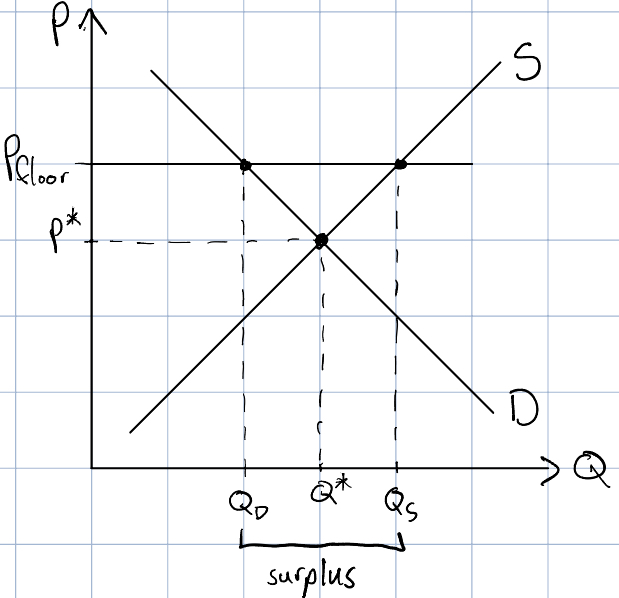
\includegraphics[width = 0.3\textwidth]{ch6_qq1}
	\end{center}
	
\item (d) --

	\begin{center}
	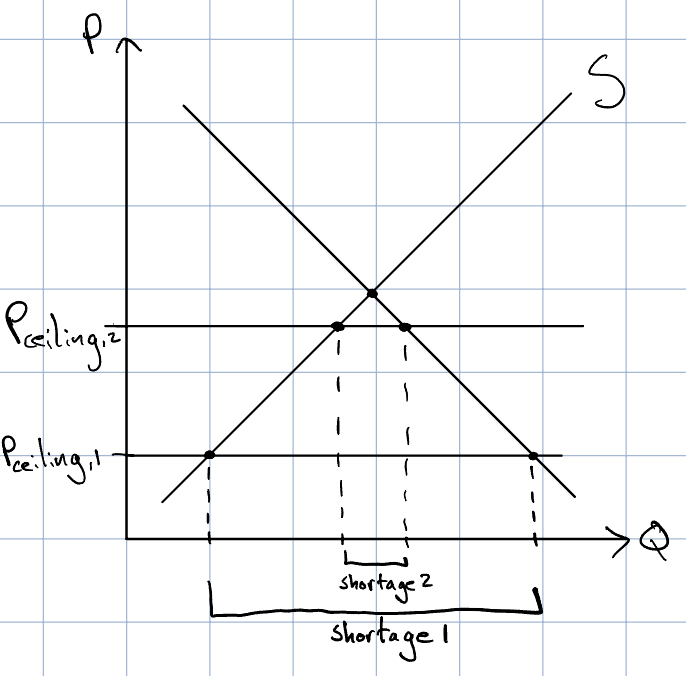
\includegraphics[width = 0.3\textwidth]{ch6_qq2}
	\end{center}
	
\item (a) -- In the long run, landlords and renters have more time to change their behavior in response to the price ceiling, so supply and demand become more elastic. That causes a larger shortage.

	\begin{center}
	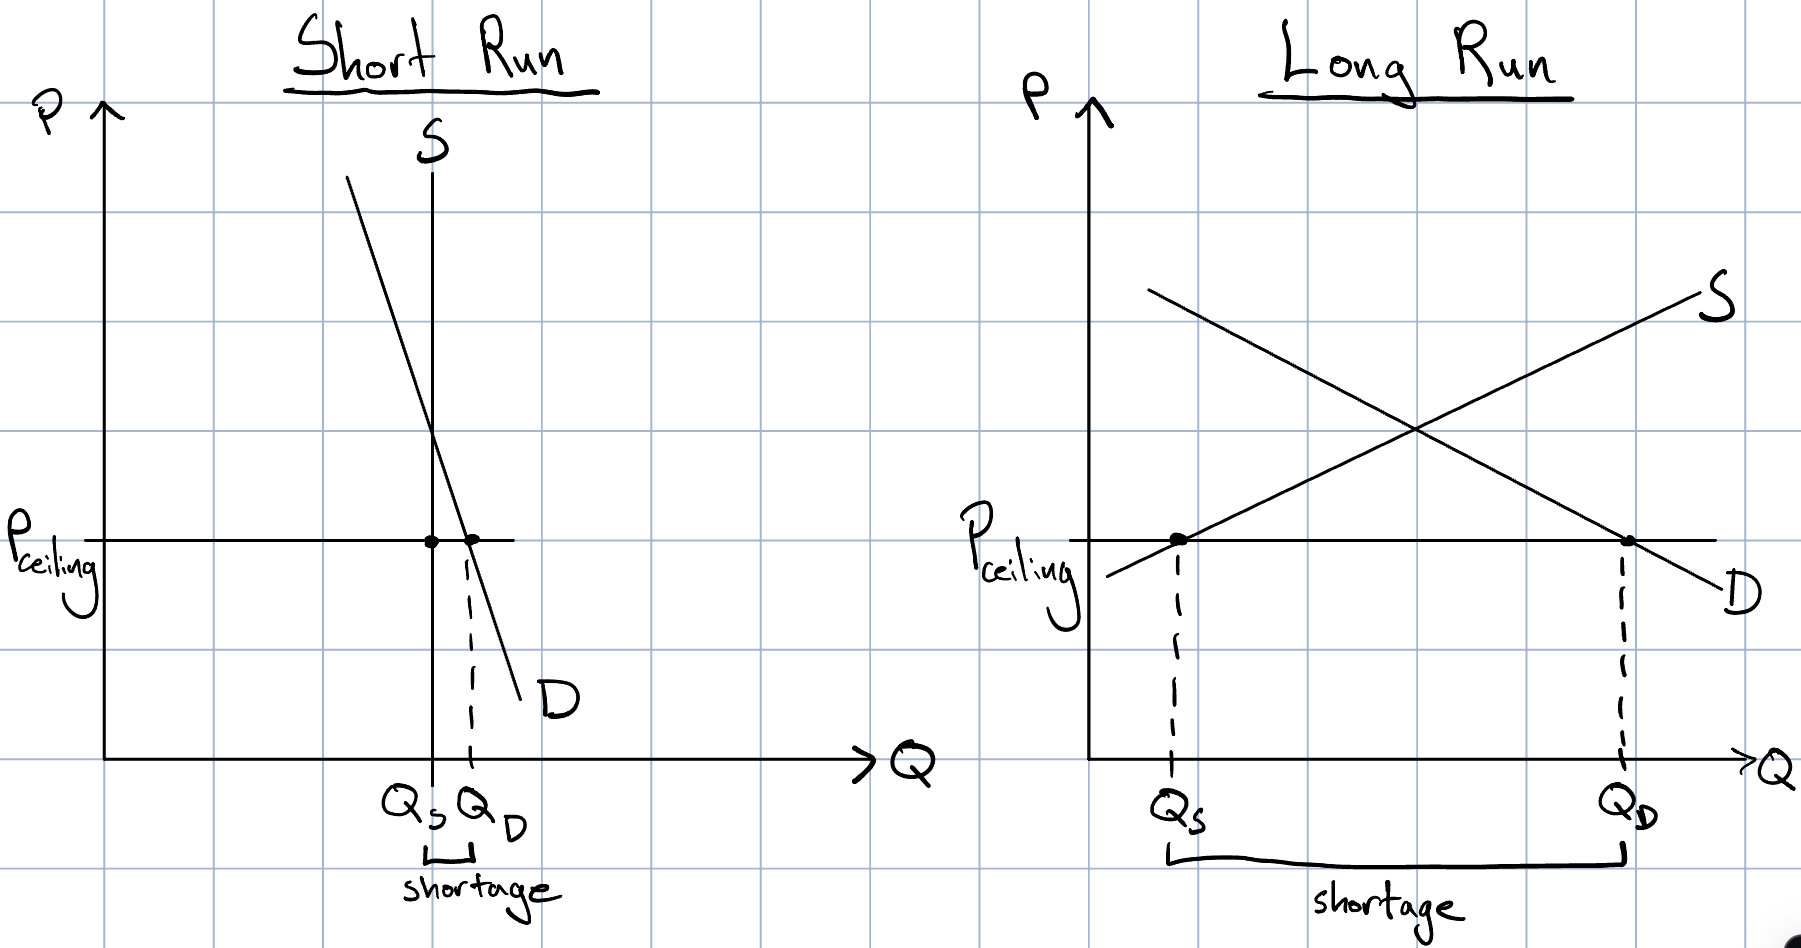
\includegraphics[width = 0.6\textwidth]{ch6_qq3}
	\end{center}

\item (c) -- Total amount paid to workers is the labor market equivalent of total expenditure. It's quantity of labor sold times the wage per unit of labor, $L \cdot W$. If demand for labor is elastic, the increase in wage will be proportionately smaller than the decrease in quantity, so total revenue will decrease.
	\begin{center}
	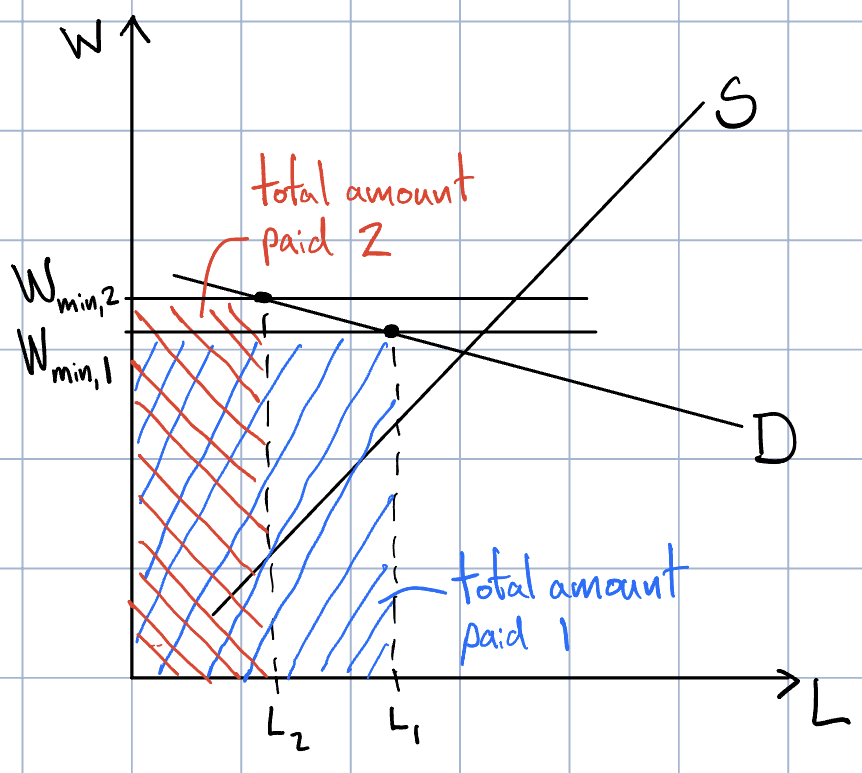
\includegraphics[width = 0.3\textwidth]{ch6_qq4}
	\end{center}
	
\item (a) -- The incidence of a tax doesn't depend on who pays the tax. It depends on the relative elasticity of supply and demand.

\item (d) -- The burden falls mainly on consumers if demand is less elastic than supply. In that case, consumers can't substitute away from consuming the good as easily as producers can substitute away from producing the good. As a result, consumers end up bearing most of the burden of the tax.

\item (c) --
	\begin{center}
	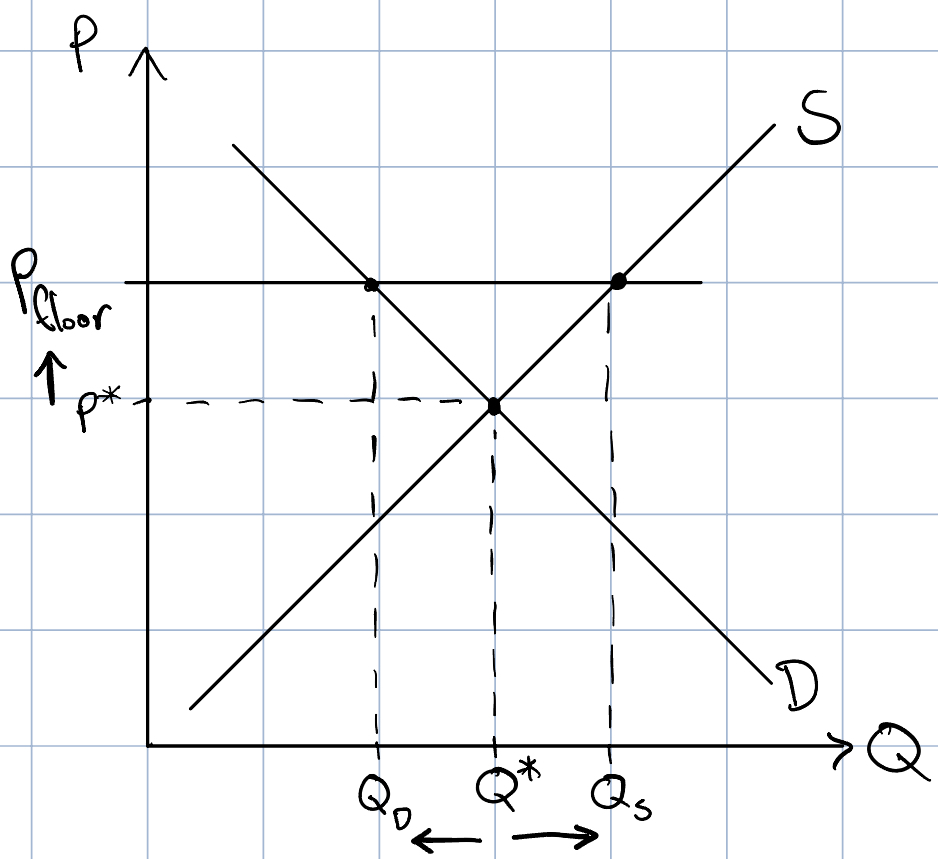
\includegraphics[width = 0.3\textwidth]{ch6_qq7}
	\end{center}
	
\item (b) --
	\begin{center}
	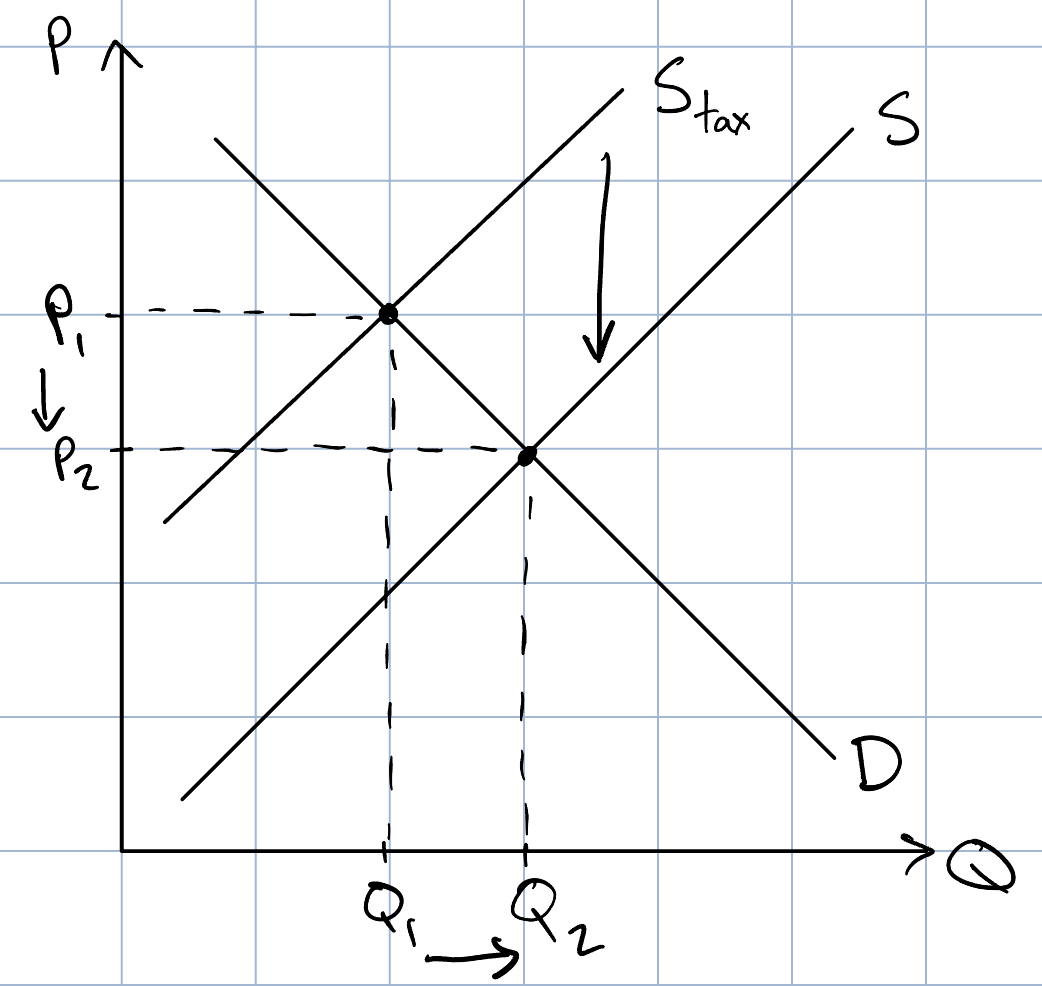
\includegraphics[width = 0.3\textwidth]{ch6_qq8}
	\end{center}
	
\end{enumerate}
	
\section*{Questions for Review}

\begin{enumerate}

\item Rent control is a price ceiling, and minimum wage is a price floor.

\item A price ceiling causes a shortage.
	\begin{center}
	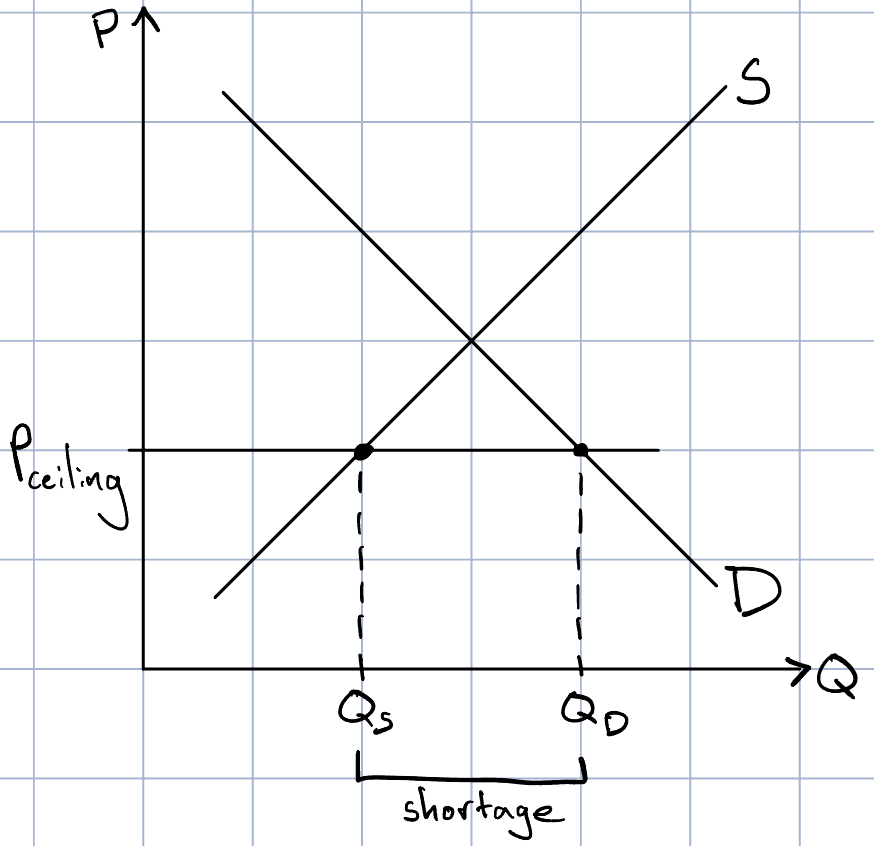
\includegraphics[width = 0.3\textwidth]{ch6_qfr2}
	\end{center}
	
\item We're not going to emphasize this in class, but when there's a shortage or a surplus, people develop some sort of rationing mechanism to determine who gets the good. Long lines, under-the-table compensation, and prejudice are all potential rationing mechanisms.

\item In a competitive market, a binding price control will reduce the quantity sold relative to the market equilibrium. That means it eliminates mutually beneficial trades that buyers and sellers would otherwise choose to make. Therefore, price controls help some people, but they hurt others who no longer get to trade the good. \textit{Importantly, this critique of price controls depends on the market being competitive. If the market isn't competitive, economists are significantly more supportive of price controls.}

\item The policy increases the price that consumers pay sellers by the amount of the tax. It does not increase the amount buyers are out pocket because the money they were giving the government is now going to the seller. It also does not change the amount that sellers receive (net taxes) because they give all of the additional money that buyers pay them to the government. The quantity sold of the good does not change.
	\begin{center}
	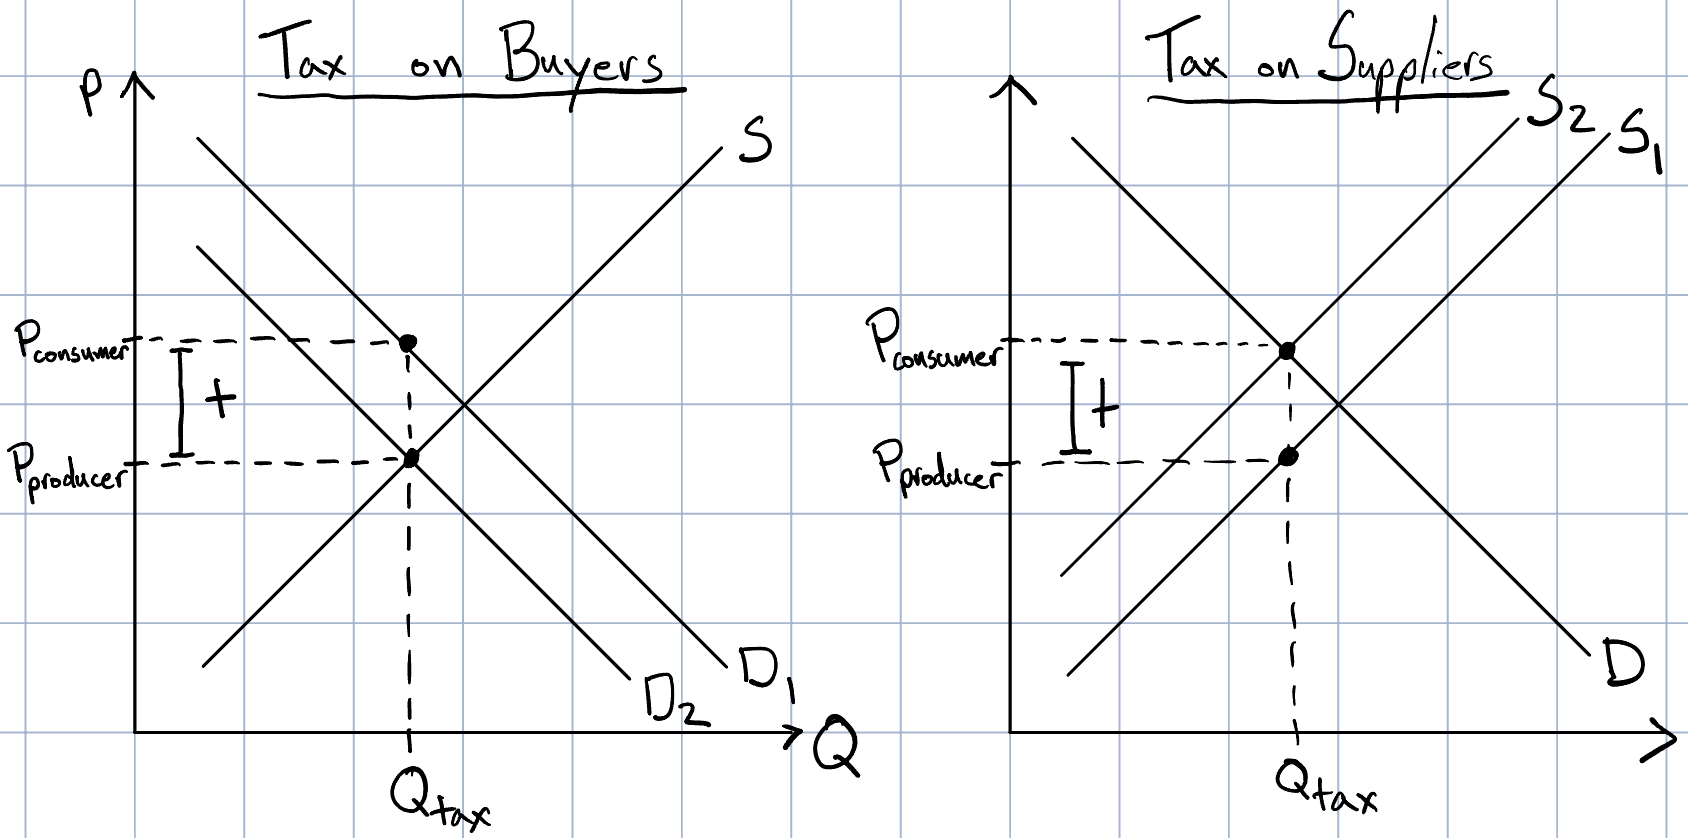
\includegraphics[width = 0.6\textwidth]{ch6_qfr5}
	\end{center}
	
\item It increases the price paid by buyers, decreases the price received by sellers, and decreases the quantity sold.
	\begin{center}
	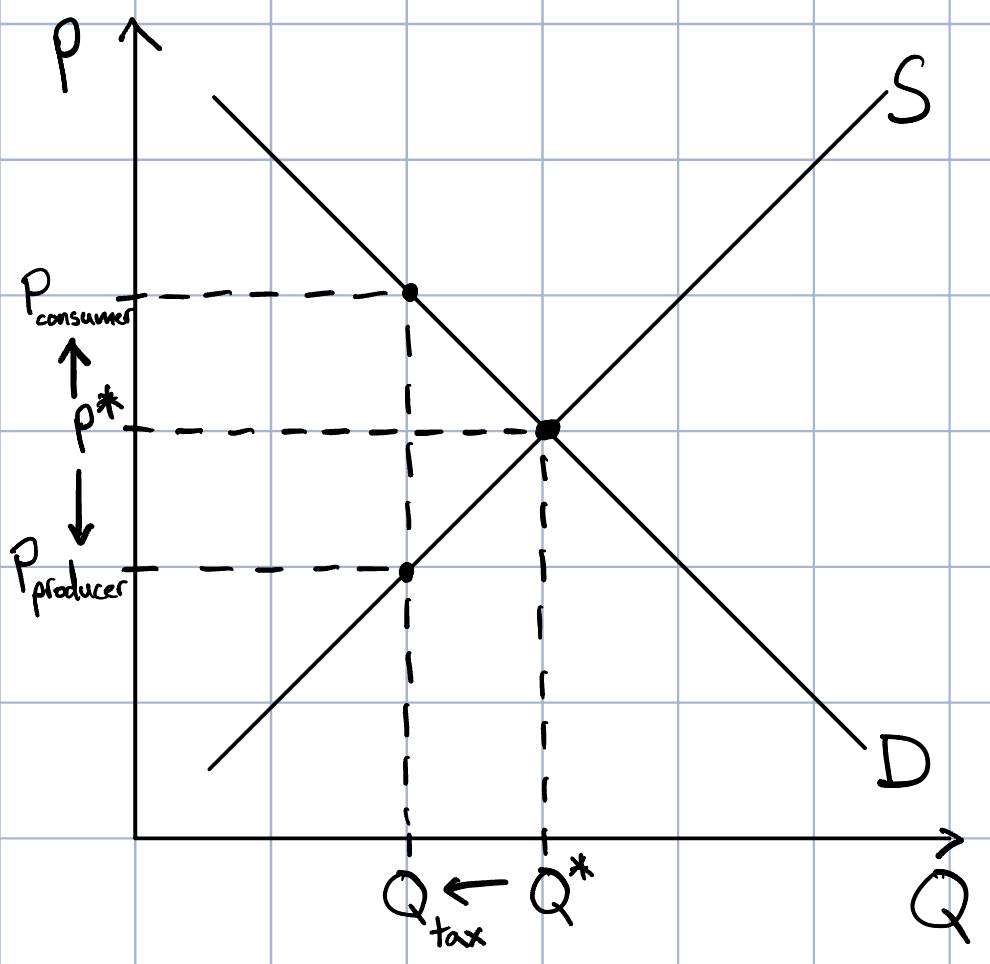
\includegraphics[width = 0.3\textwidth]{ch6_qfr6}
	\end{center}
	
\item The relative elasticity of supply and demand determines how the burden of a tax is divided between buyers and sellers. The relative elasticity tells us whether buyers or sellers can more easily change their behavior and leave the market. Whichever group is less able to change and leave the market ends up bearing more of the burden. 

\end{enumerate}
	
\section*{Problems and Applications}

\begin{enumerate}

\item If the price ceiling is non-binding, then the price ceiling has no effect because the price remains the same after the policy. If the price ceiling is binding, the number of people attending comedy shows decreases because the quantity of comedy performances supplied decreases.
	\begin{center}
	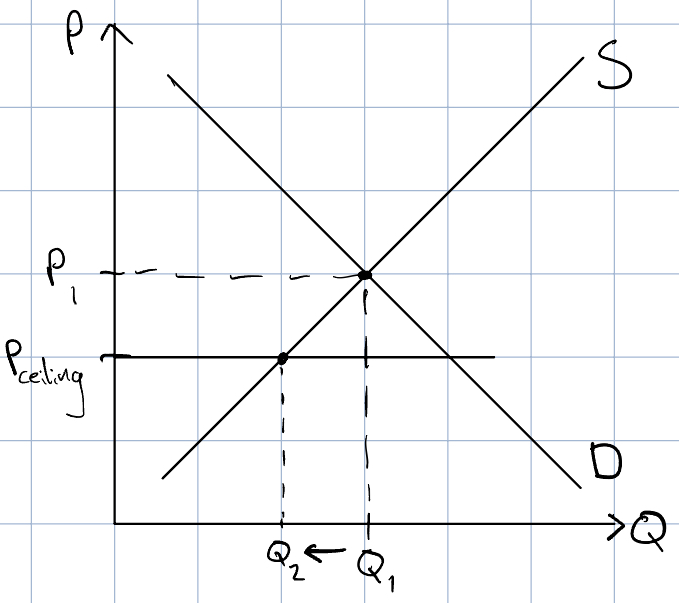
\includegraphics[width = 0.3\textwidth]{ch6_paa1}
	\end{center}
	
\item

	\begin{enumerate}
	
	\item There is a surplus. 
	
		\begin{center}
		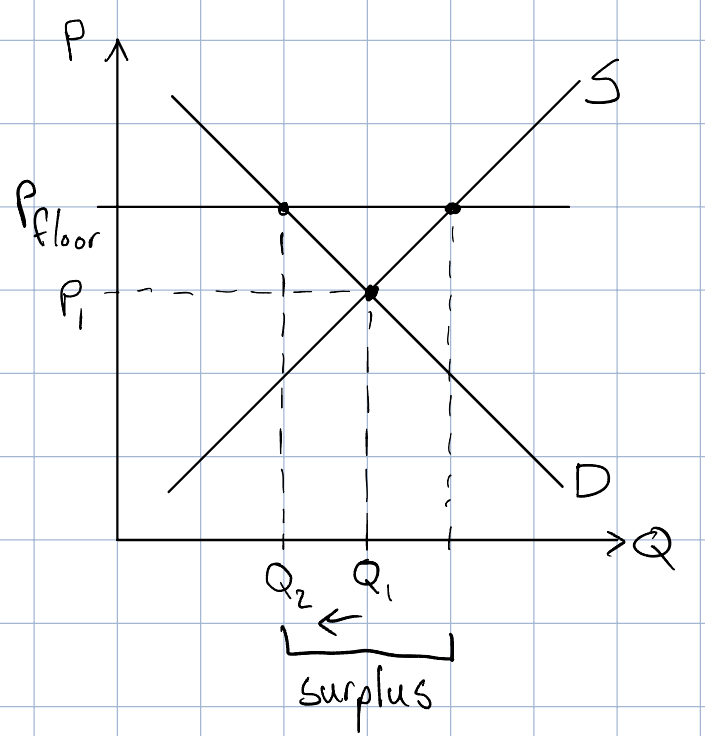
\includegraphics[width = 0.3\textwidth]{ch6_paa2a}
		\end{center}
	
	\item Yes, if demand is elastic, then the increase in price will be proportionately smaller than the decrease in quantity.
	
		\begin{center}
		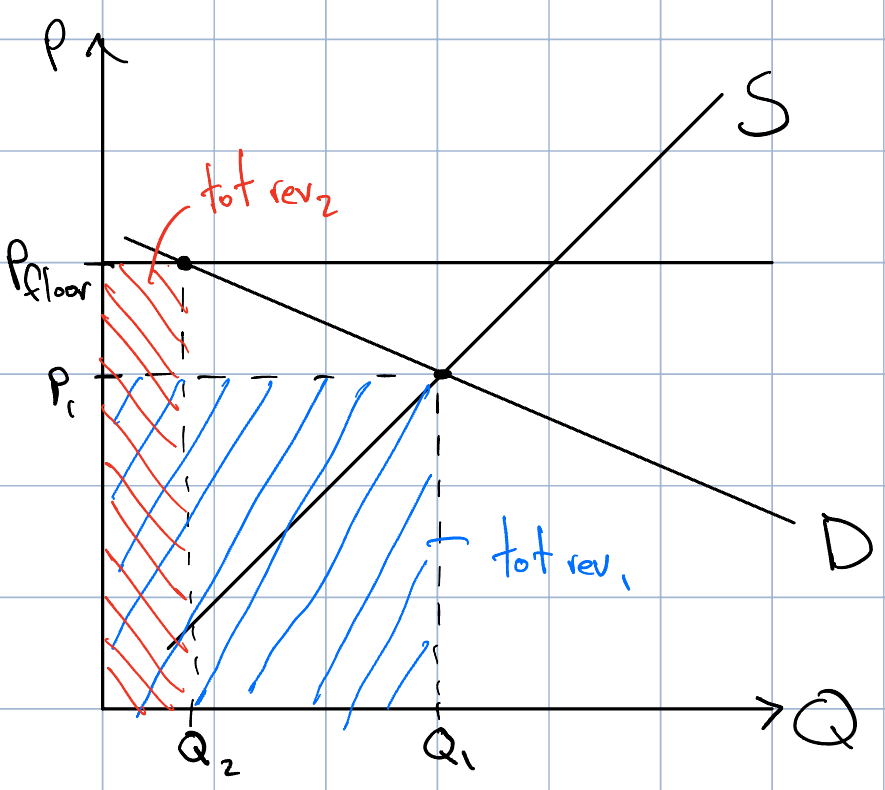
\includegraphics[width=0.3\textwidth]{ch6_paa2b}
		\end{center}
	
	\item All of the producers who couldn't find a buyer at the basic price floor benefit. Tax payers lose because the government has to spend money (raised through taxes) on cheese that buyers don't want to buy at that price.
	
	\end{enumerate}
	

\item

	\begin{enumerate}
	
	\item $Q^* = 6$ million and $P^* = \$8$ because $Q_S = Q_D$ when $P = \$8$.
	
	\item $P_{Floor} = \$10$. The quantity sold is the minimum of $Q_D$ and $Q_S$ because you can't force buyers to buy more than they want and you can't force sellers to sell more than they want. Since this price floor is above the equilibrium price, quantity demanded is lower than quantity supplied, and 2 million frisbees are sold.
	
	\item $P_{Ceiling} = \$9$. $P_{Ceiling} > P^*$ which means the price ceiling is non-binding. Therefore, the market moves towards equilibrium. The market price goes back to \$8, and 6 million frisbees are sold. 
	
	\end{enumerate}
	
\item 

	\begin{enumerate}
	
	\item At the market equilibrium, there is no difference between the price paid by consumers and the price received by sellers. 
		\begin{center}
		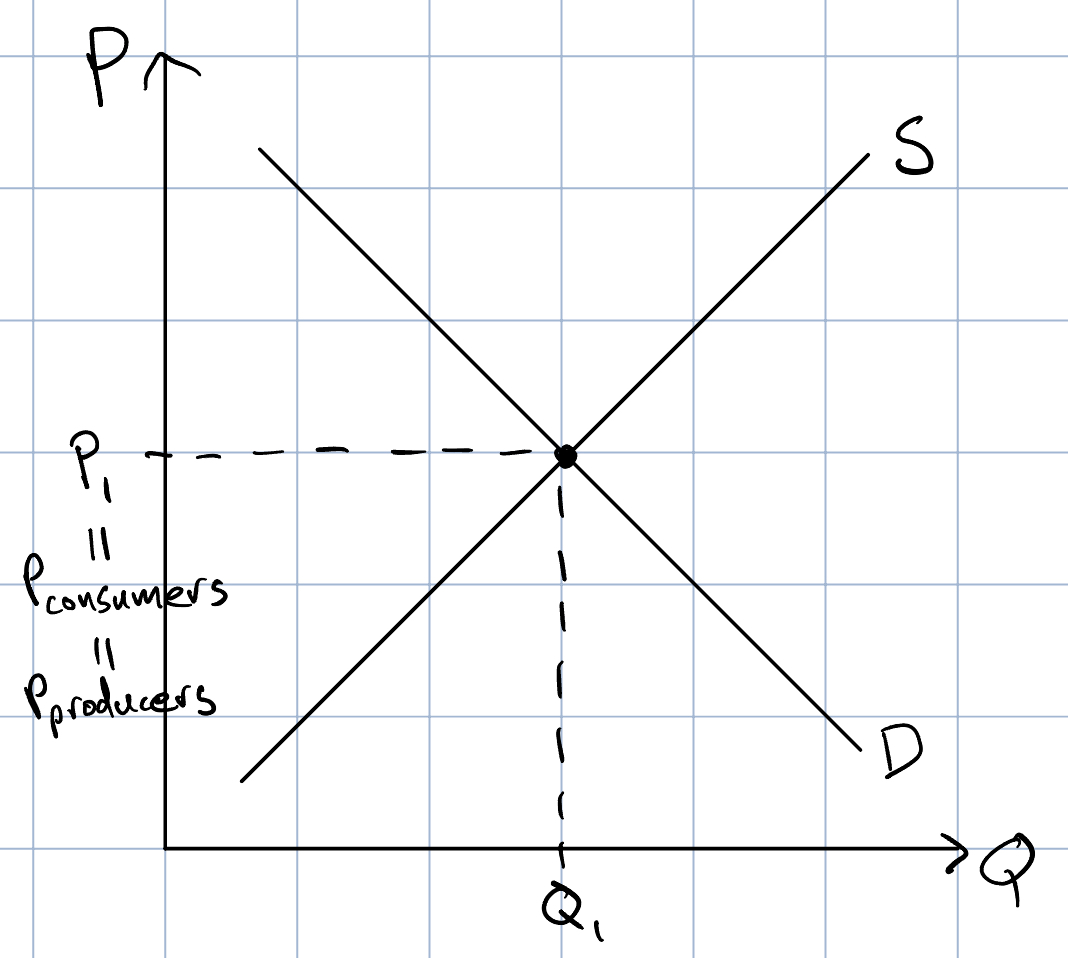
\includegraphics[width = 0.3\textwidth]{ch6_paa4a}
		\end{center}
	
	\item The difference between the price paid by consumers and the price received by sellers is the amount of the tax, \$2. The quantity of beer sold has decreased.
		\begin{center}
		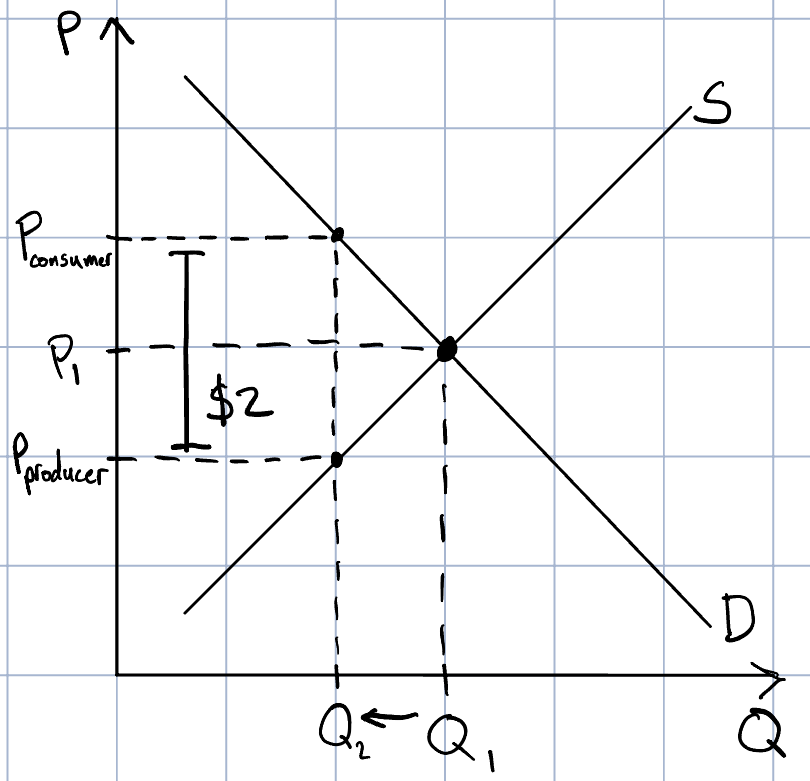
\includegraphics[width = 0.3\textwidth]{ch6_paa4b}
		\end{center}
	
	\end{enumerate}
	
\item The question says the policy would use \underline{part} of the extra revenue to reduce the payroll tax paid by workers. I interpret that to mean the policymakers plan to have new revenue left over after reducing the workers' payroll tax. If that's the case, then the policymakers must be increasing the overall tax rate in addition to shifting the amount paid by firms relative to workers. That's all to say, I understand the policy to have two components -- make firms pay more of the tax and increase the tax overall.

The tax would likely achieve its first goal of raising revenue. Labor demand and supply are likely inelastic (at least in the short run), so a higher tax won't decrease the quantity of labor sold very much. If the tax rate rises and the quantity sold doesn't decrease much, tax revenue should increase.
	\begin{center}
	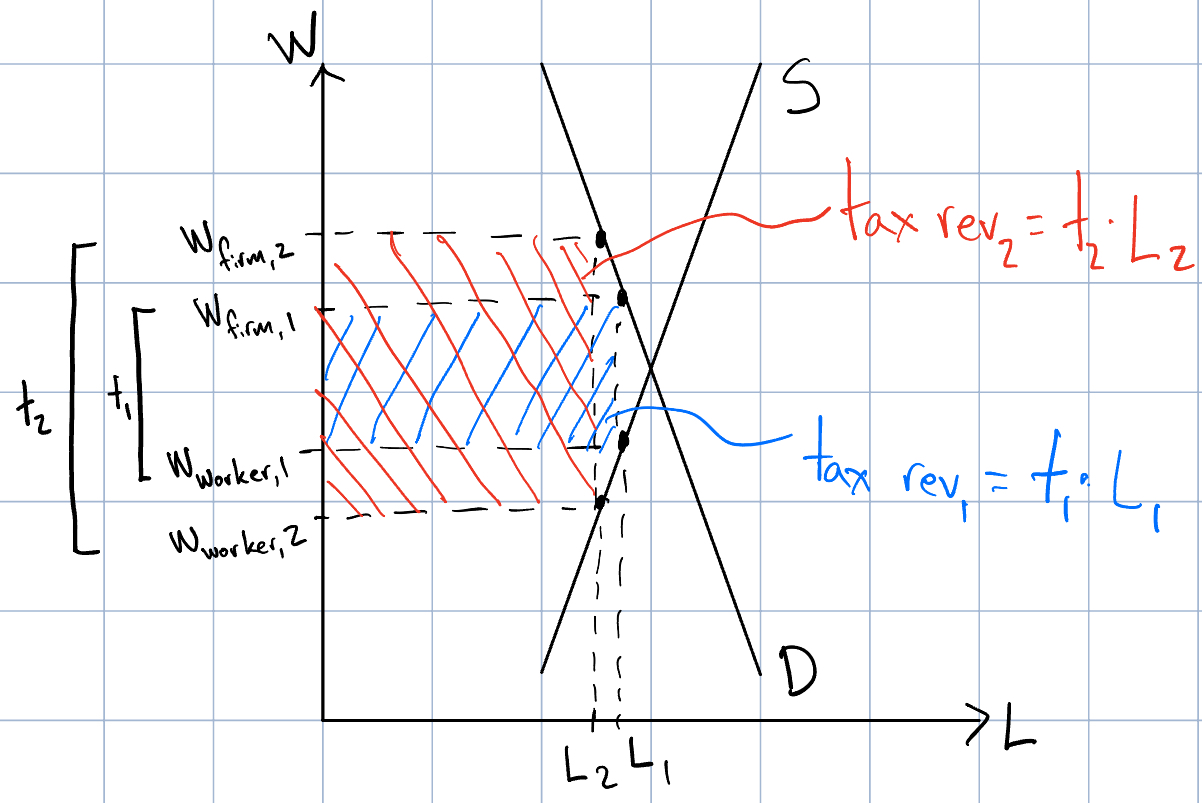
\includegraphics[width = 0.45\textwidth]{ch6_paa5_1}
	\end{center}
	
That said, the tax wouldn't make workers better off. Who pays a tax doesn't determine the incidence of a tax. The elasticity of supply and demand determine the incidence of a tax. Since the policy does nothing to affect those two elasticities, it won't shift the incidence towards firms and away from workers. The tax increase will decrease the quantity of labor sold and decrease the wage workers receive, so it will actually make workers worse off.

\item It will rise by less than \$500. The incidence of the tax will be split between consumers and producers. Since, demand for luxury cars is likely highly elastic, more of the tax burden is likely to fall on producers.
	
\item 

	\begin{enumerate}
	
	\item It doesn't matter who congress imposes the tax on. Whether they impose it on producers or consumers, the decrease in quantity and the incidence of the tax will remain the same.
		\begin{center}
		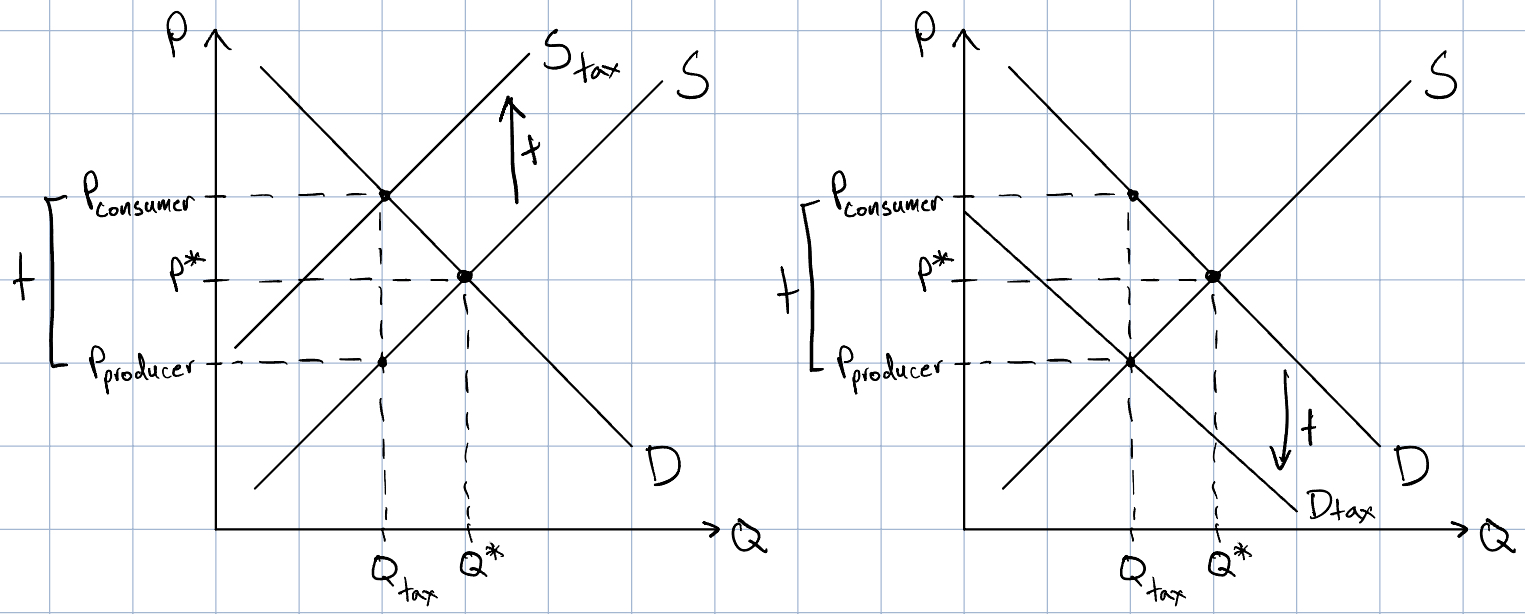
\includegraphics[width = 0.6\textwidth]{ch6_paa7a}
		\end{center}
		
	\item The tax increases the price that consumers pay for gasoline. If demand were more elastic, consumers would respond to that price increase by decreasing their quantity demanded more. Therefore, the policy would be more effective.
		\begin{center}
		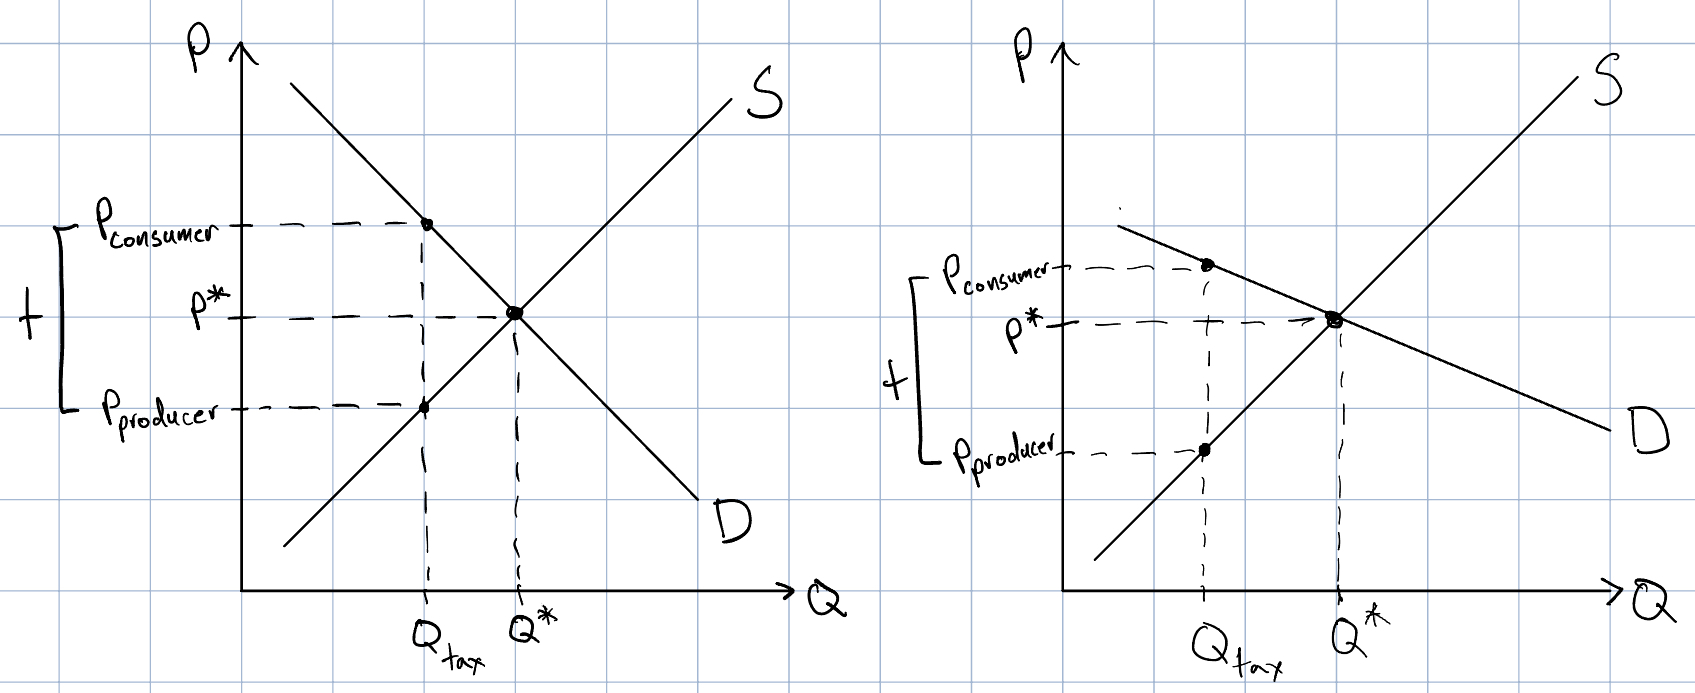
\includegraphics[width = 0.6\textwidth]{ch6_paa7b}
		\end{center}
		
	\item It depends on how much producers value the decline in air pollution and how much they value the government's use of its new tax revenue. Consumers buy less and pay more for gas after the tax, so they're hurt in the gas market. That said, if they value clean air and whatever project the government funds with its new revenue more than they value cheap gas, then they end up better off.
	
	\item Producers are in the same situation as consumers -- it depends. They sell a smaller quantity and receive a lower price for their gas after the tax, so they're hurt in the gas market. If they value clean air and the government's use of its new revenue more than they value better gas sales, they end up better off. 
	
	\end{enumerate}

\item

	\begin{enumerate}
	
	\item \phantom{x}
	
		\begin{center}
		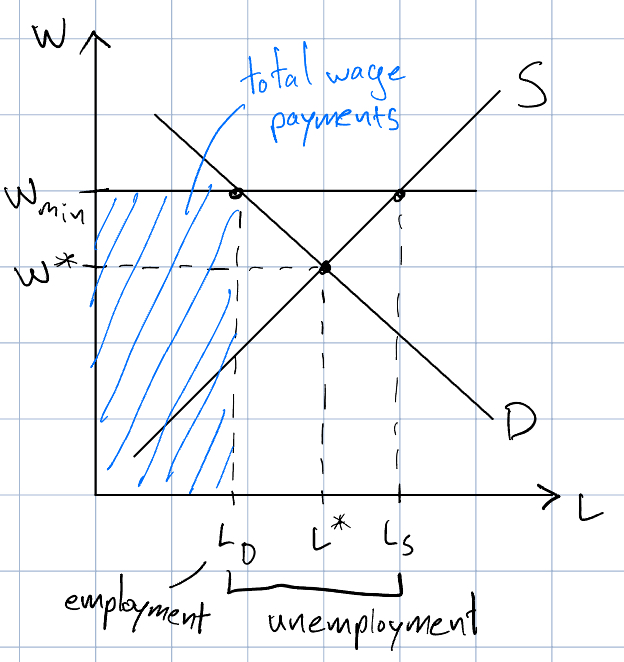
\includegraphics[width = 0.3\textwidth]{ch6_paa8a}
		\end{center}
		
	\item The increase in the minimum wage would decrease employment because the quantity of labor demanded would decrease. Only the price elasticity of demand affects the change in employment because the slope of the demand curve determines how the quantity of labor demanded changes when wage increases.
		\begin{center}
		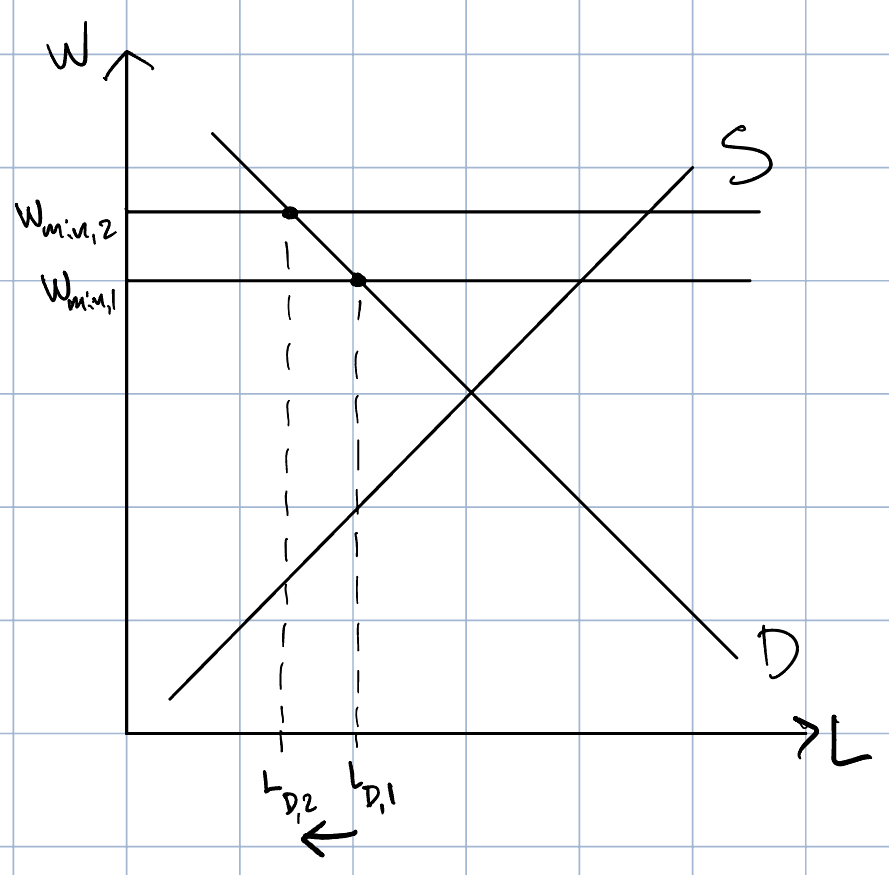
\includegraphics[width = 0.3\textwidth]{ch6_paa8b}
		\end{center}
		
	\item The increase in the minimum wage would increase unemployment because the quantity of labor demanded would decrease at the same time that the quantity of labor supplied would increase. Both the price elasticity of demand and supply affect the change in unemployment. The slope of the demand curve determines how the quantity of labor demanded changes when wage increases. The slope of the supply curve determines how the quantity of labor supplied changes when wage increases. 
	\begin{center}
	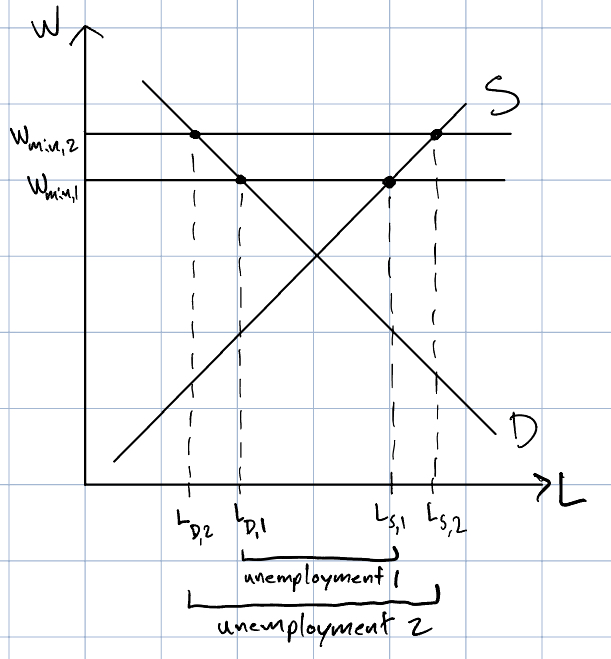
\includegraphics[width = 0.3\textwidth]{ch6_paa8c}
	\end{center}
	
	\item If labor demand were inelastic, the minimum wage increase would increase total wage payments because the decrease in employment would be proportionately smaller than the increase in wages. If labor demand were elastic, the minimum wage increase would decrease total wage payments because the decrease in employment would be proportionately larger than the increase in wages. 
	\begin{center}
	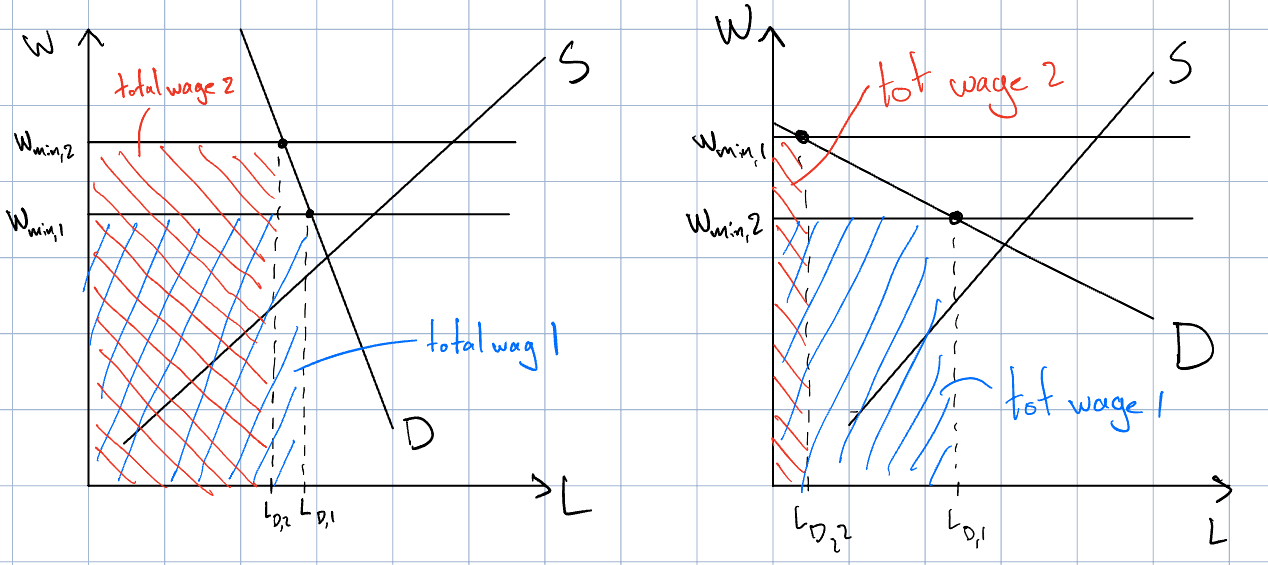
\includegraphics[width = 0.6\textwidth]{ch6_paa8d}
	\end{center}
	
	\end{enumerate}
	
\item The tax burden falls entirely on the team owners because their supply of seats is perfectly inelastic. When demand shifts down, the price that consumers pay doesn't move at all, and the price that producers receive goes down by \$5, the full amount of the tax.
	\begin{center}
	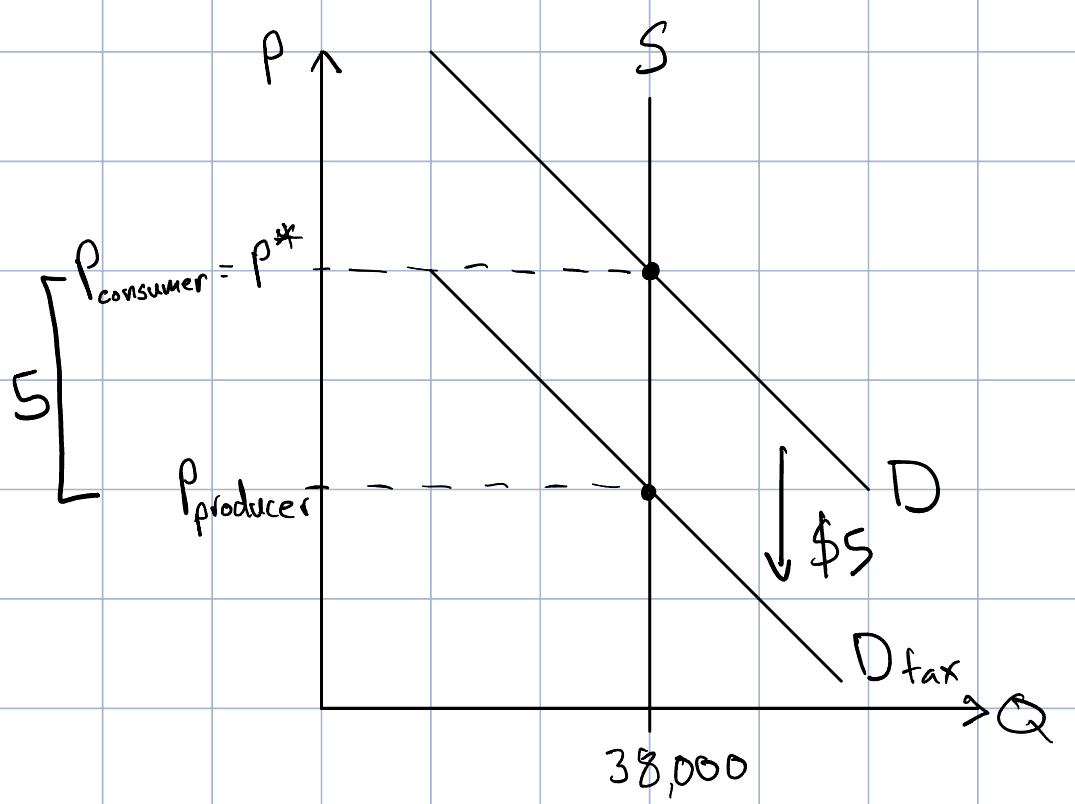
\includegraphics[width = 0.3\textwidth]{ch6_paa9}
	\end{center}
	
\item
	\begin{enumerate}
	
	\item
		\begin{align*}
		Q_S &= Q_D \\
		2P^* &= 300 - P^* \\
		3P^* &= 300 \\
		P^* &= 100 \\
		Q^* &= 2P^* = 2(100) = 200 
		\end{align*}
		
	\item A shortage develops because the price ceiling is binding. Therefore, $P = P_{ceiling} = 90$. 
		\begin{align*}
		Q_S &= 2P_{ceiling} = 2(90) = 180 \\
		Q_D &= 300 - P_{ceiling} = 300 - 90 = 210 \\
		Shortage &= Q_D - Q_S = 210 - 180 = 30
		\end{align*}
		
		\begin{center}
		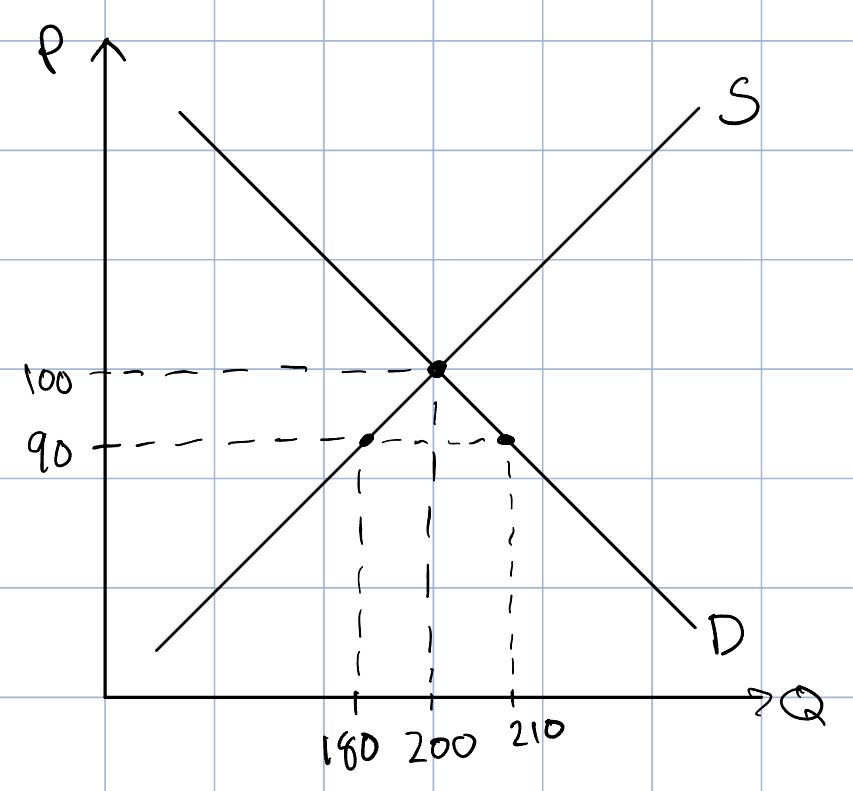
\includegraphics[width = 0.3\textwidth]{ch6_paa10b}
		\end{center}
		
	\item Neither develops because the price floor isn't binding. Therefore, $P = P^* = 100$, and $Q_S = Q_D = Q^* = 200$.
	
	\item No shortage or surplus develops.
		\begin{align*}
		Q_D &= 300 - P_{consumer} \\
		Q_S &= 2(P_{consumer} - 30) = 2P_{consumer} - 60 \\
		300 - P_{consumer} &= 2P_{consumer} - 60 \\
		360 &= 3P_{consumer} \\
		120 &= P_{consumer} \\
		P_{producer} &= P_{consumer} - 30 = 120 - 30 = 90 \\
		Q_{tax} &= Q_S = Q_D = 300 - 120 = 180
		\end{align*}
		
		\begin{center}
		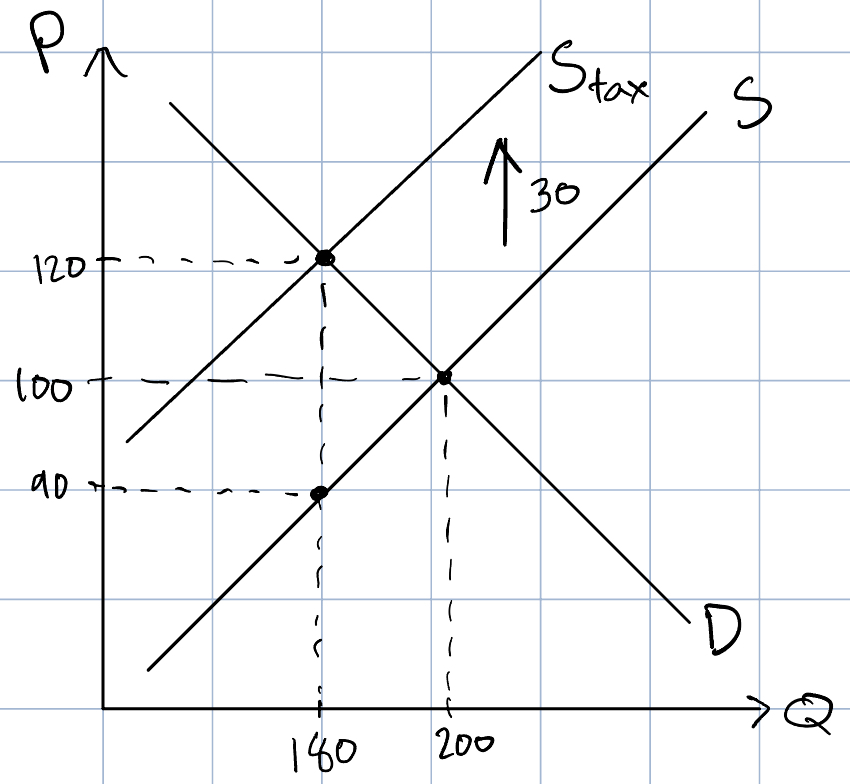
\includegraphics[width = 0.3\textwidth]{ch6_paa10d}
		\end{center}
	
	\end{enumerate}
	
\end{enumerate}
	
\section*{Non-Textbook Questions}

\begin{enumerate}

\item \begin{align*}
	2,500 - 3P^* &= 5P^* - 100 \\
	2,600 &= 8P^* \\
	325 &= P^* \\
	Q^* &= 5(325) - 100 = 1,525 \\
	Q_{ceiling} &= 5P_{ceiling} - 100 = 5(300) - 100 = 1,400 \\
	\Delta Q &= Q_{ceiling} - Q^* = 1,400 - 1,525 = -125
	\end{align*}
	
	\begin{center}
	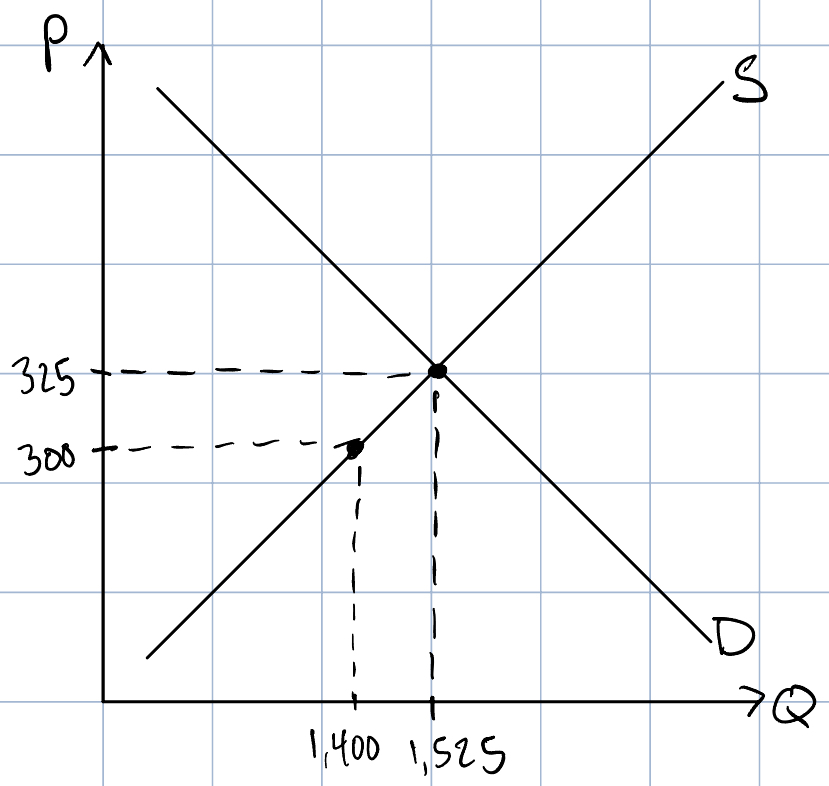
\includegraphics[width = 0.3\textwidth]{ch6_ntq1}
	\end{center}
	
\item 
	\begin{enumerate}
	
	\item \begin{align*}
		Q_D &= Q_S \\
		150 - 5P^* &= 5P^* \\
		150 &= 10P^* \\
		15 &= P^* \\
		Q^* &= 5P^* = 5(15) =  75 \\
		Q_{floor} &= 150 - 5P_{floor} = 150 - 5(20) = 50 \\
		\Delta Q &= Q_{floor} - Q^* = 50 - 75 = -25
		\end{align*}
		
		\begin{center}
		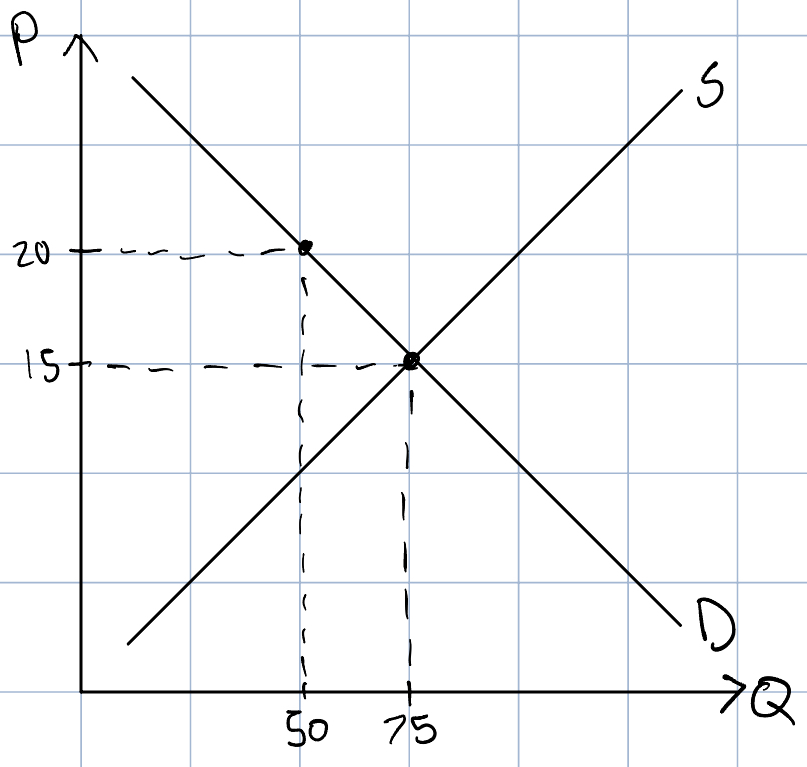
\includegraphics[width = 0.3\textwidth]{ch6_ntq2a}
		\end{center}
	
	\item \phantom{x}
		\begin{center}
		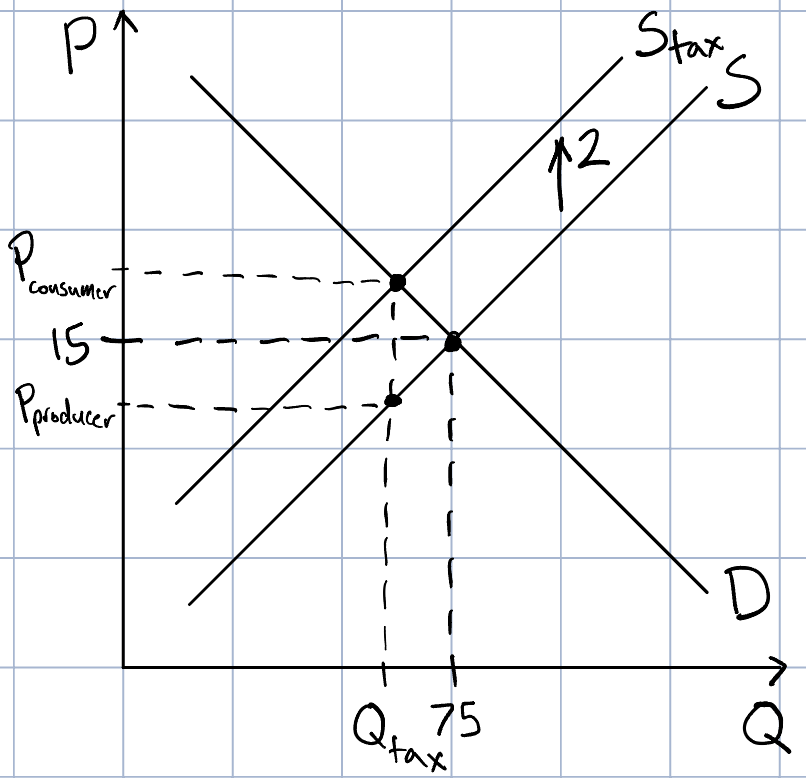
\includegraphics[width = 0.3\textwidth]{ch6_ntq2b}
		\end{center}
	
		 Invert supply and demand:
		\begin{align*}
		Q_D &= 150 - 5P \\
		5P &= 150 - Q_D \\
		P &= 30 - \frac{1}{5}Q_D \\
		\\
		Q_S &= 5P \\
		P &= \frac{1}{5}Q_S
		\end{align*}
		Find new supply curve by translating the original up by 2:
		\begin{equation*}
		P = \frac{1}{5}Q_S + 2
		\end{equation*}
		Find new equilibrium quantity:
		\begin{align*}
		30 - \frac{1}{5}Q &= \frac{1}{5}Q + 2 \\
		28 &= \frac{2}{5}Q \\
		70 &= Q_{tax}
		\end{align*}
		Find change in quantity:
		\begin{equation*}
		\Delta Q = Q_{tax} - Q^* = 70 - 75 = -5
		\end{equation*}
		
	\item There's no meaningful difference between a tax on consumers and a tax on producers, so we can use the graph, inverse equations, and $Q_{tax}$ we found in part (b).
	
		First, we find the price consumers pay and the price producers take home:
		\begin{align*}
		P_{consumer} &= 30 - \frac{1}{5}Q_{tax} \\
		&= 30 - \frac{1}{5}(70) \\
		&= 16 \\
		P_{producer} &= P_{consumer} - 2 \\
		&= 16 - 2 \\
		&= 14
		\end{align*}
		
		Then, we find consumers' and producers' share of the tax:
		\begin{align*}
		\text{Consumer: }& \frac{P_{consumer} - P^*}{t} \cdot 100 = \frac{16 - 15}{2} \cdot 100 = 50\% \\
		\text{Producer: }& 100\% - 50\% = 50\%
		\end{align*}
	
	\end{enumerate}
	
%\item
%	\begin{enumerate}
%	
%	\item
%		\begin{align*}
%		600 - 150P^* &= 200P^* - 100 \\
%		700 &= 350P^* \\
%		2 &= P^* \\
%		Q^* &= 600 - 150(2) \\
%		&= 300
%		\end{align*}
%	
%	\item \phantom{x}
%		\begin{center}
%		\includegraphics[width = 0.3\textwidth]{ch6_ntq3b}
%		\end{center}
%		
%		\begin{align*}
%		Q_S &= 200P_{producer} - 100 \\
%		Q_D &= 600 - 150(P_{producer} + 0.875) = 468.75 - 150P_{producer} \\
%		200P_{producer} - 100 &= 468.75 - 150P_{producer} \\
%		350P_{producer} &= 568.75 \\
%		P_{producer} &= 1.625 \\
%		P_{consumer} &= P_{producer} + 0.875 = 1.625 + 0.875 = 2.50
%		\end{align*}
%		
%		Inverse supply and demand:
%		\begin{align*}
%		Q_D &= 600 - 150P \\
%		150P &= 600 - Q_D \\
%		P &= 4 - \frac{1}{150}Q_D \\
%		\\
%		Q_S &= 200P - 100 \\
%		200P &= Q_S + 100 \\
%		P&= \frac{1}{200} Q_S + \frac{1}{2}
%		\end{align*}
%		
%		After-tax demand:
%		\begin{align*}
%		P &= 4 - \frac{1}{150}Q_D - 0.875\\
%		&= 3.125 - \frac{1}{150}Q_D
%		\end{align*}
%		
%		After-tax quantity:
%		\begin{align*}
%		3.125 - \frac{1}{150}Q &= \frac{1}{200}Q + \frac{1}{2} \\
%		3.625 &= \frac{7}{600}Q \\
%		
%		\end{align*}
%		
%	\item $Q_{tax} = 200P_{producer} - 100 = 200(1.625) - 100 = 225$
%	
%	\end{enumerate}

\item
	\begin{enumerate}
	
	\item Pre-tax equilibrium:
		\begin{align*}
		100 - 2P &= -20 + 4P \\
		120 &= 6P \\
		20 &= P^* \\
		Q^* &= 100 - 2P^* \\
		&= 60
		\end{align*}
		
		Inverse supply and demand:
		\begin{align*}
		Q_D &= 100 - 2P \\
		2P &= 100 - Q_D \\
		P &= 50 - \frac{1}{2}Q_D \\
		\\
		Q_S &= -20 + 4P \\
		4P &= Q_S + 20 \\
		P &= \frac{1}{4}Q_S + 5 \\
		\end{align*}
		
		After-tax demand: \\
		It doesn't matter whether we model the tax on producers or consumers, so I'm arbitrarily going to pick consumers.
		\begin{center}
		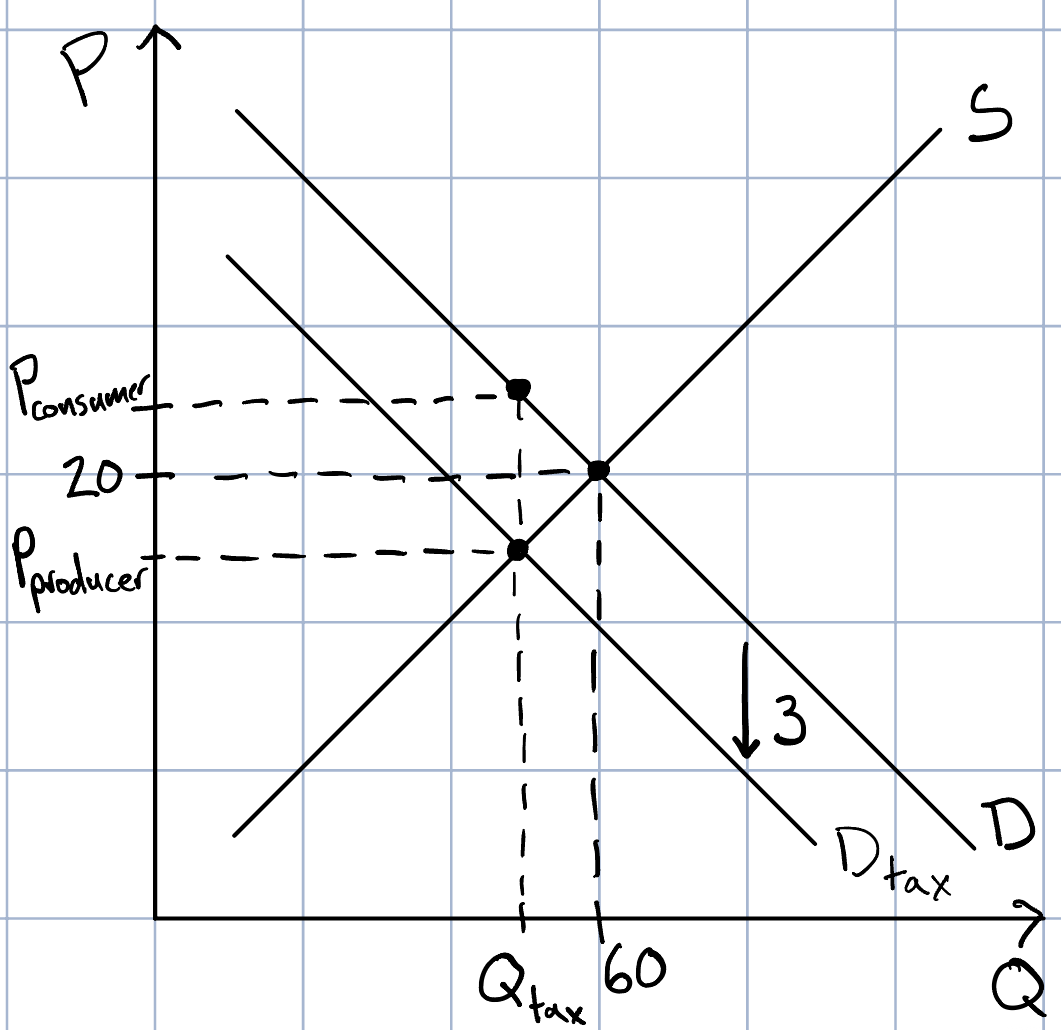
\includegraphics[width = 0.3\textwidth]{ch6_ntq3a}
		\end{center}
		\begin{align*}
		P &= 50 - \frac{1}{2}Q_D - 3 \\
		&= 47 - \frac{1}{2}Q_D
		\end{align*}
		
		After-tax quantity:
		\begin{align*}
		47 - \frac{1}{2}Q &= \frac{1}{4}Q + 5 \\
		42 &= \frac{3}{4}Q \\
		56 &= Q_{tax}
		\end{align*}
		
		Change in quantity:
		\begin{equation*}
		\Delta Q = Q_{tax} - Q^* = 56 - 60 = 4
		\end{equation*}
		
	\item \begin{align*}
		P_{producer} &= \frac{1}{4}Q_{tax} + 5 \\
		&= \frac{56}{4} + 5 \\
		&= 19 \\
		P_{consumer} &= P_{producer} + 3 \\
		&= 22
		\end{align*}
		
		Consumer share:
		\begin{equation*}
		\frac{P_{consumer} - P^*}{3} \cdot 100 = 66.67\%
		\end{equation*}
		
		Producer share:
		\begin{equation*}
		100\% - 66.67\% = 33.33\%
		\end{equation*}
		
	\item Supply is more elastic than demand because producers bear less of the burden of the tax.
	
	\end{enumerate}
	
\item
	\begin{enumerate}
	
	\item \begin{align*}
		50 - 2W &= -10 + 2W \\
		60 &= 4W \\
		15 &= W^* \\
		L^* &= 50 - 2W^* \\
		&= 20
		\end{align*}
		
	\item \phantom{x}
		\begin{center}
		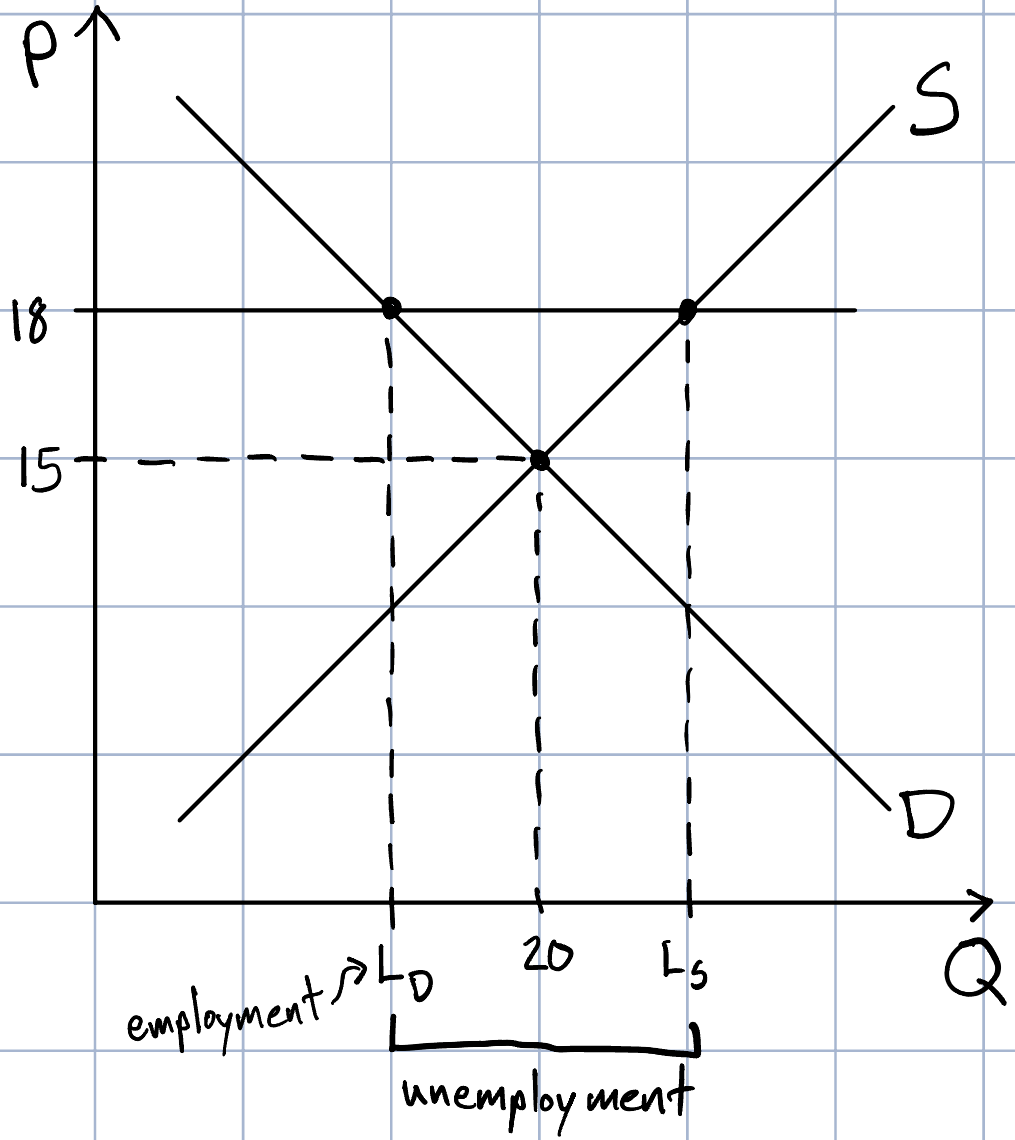
\includegraphics[width = 0.3\textwidth]{ch6_ntq4b}
		\end{center}
	
		\begin{align*}
		E &= L_D \\
		&= 50 - 2(18) \\
		&= 14
		\end{align*}
		
	\item \begin{align*}
		L_S &= -10 + 2(18) \\
		&= 26 \\
		U &= L_S - L_D \\
		&= 26 - 14 \\
		&= 12
		\end{align*}
	
	\end{enumerate}

\end{enumerate}

\end{document}